%!TEX root = index.tex
\section[Resultados]{Resultados}
\begin{frame}
\frametitle{Resultados}
Aquisição de dados

\begin{equation} 
\mathbf{A} = 
\begin{bmatrix} 
 a_{i_1 f_1} &  a_{i_1 f_2} &  a_{i_1 f_3}  & \dots   \\
 a_{i_2 f_1} &  a_{i_2 f_2} &  a_{i_2 f_3}  & \dots   \\
 a_{i_3 f_1} &  a_{i_3 f_2} &  a_{i_3 f_3}  & \dots  \\ 
 \vdots &  \vdots &  \vdots  & \ddots   \\
 \end{bmatrix}
\end{equation}

\begin{equation}
	\mathbf{B} = 
\begin{bmatrix} 
 b_{u_1 c_1} &  b_{u_1 c_2} &  b_{u_1 c_3}  & \dots   \\
 b_{u_2 c_1} &  b_{u_2 c_2} &  b_{u_2 c_3}  & \dots   \\
 b_{u_3 c_1} &  b_{u_3 c_2} &  b_{u_3 c_3}  & \dots  \\ 
 \vdots &  \vdots &  \vdots  & \ddots   \\
 \end{bmatrix}
\end{equation}

\begin{equation}
	  \mathbf{R} = 
\begin{bmatrix} 
  r_{u_1 i_1} &  r_{u_1 i_2} &  r_{u_1 i_3}  & \dots   \\
 r_{u_2 i_1} &  r_{u_2 i_2} &  r_{u_2 i_3}  & \dots   \\
 r_{u_3 i_1} &  r_{u_3 i_2} &  r_{u_3 i_3}  & \dots  \\ 
 \vdots &  \vdots &  \vdots  & \ddots   \\
\end{bmatrix}
\end{equation}
\end{frame}

\begin{frame}
\frametitle{Resultados}
\begin{equation} 
\mathbf{H} =
\begin{bmatrix} 
 r_{u_1 i_1} &  \theta_{h_1 1} &  \theta_{h_1 2} & \dots   \\
 r_{u_1 i_2} &  \theta_{h_2 1} &  \theta_{h_2 2} & \dots   \\
 r_{u i} &  \theta_{h 1} &  \theta_{h 2} & \dots   \\
 \vdots &  \vdots &  \vdots  & \ddots   \\
 \end{bmatrix} 
\end{equation}
\end{frame}

\begin{frame}
\frametitle{Resultados}
Aquisição de dados

\begin{center}
\begin{figure}[ht]
    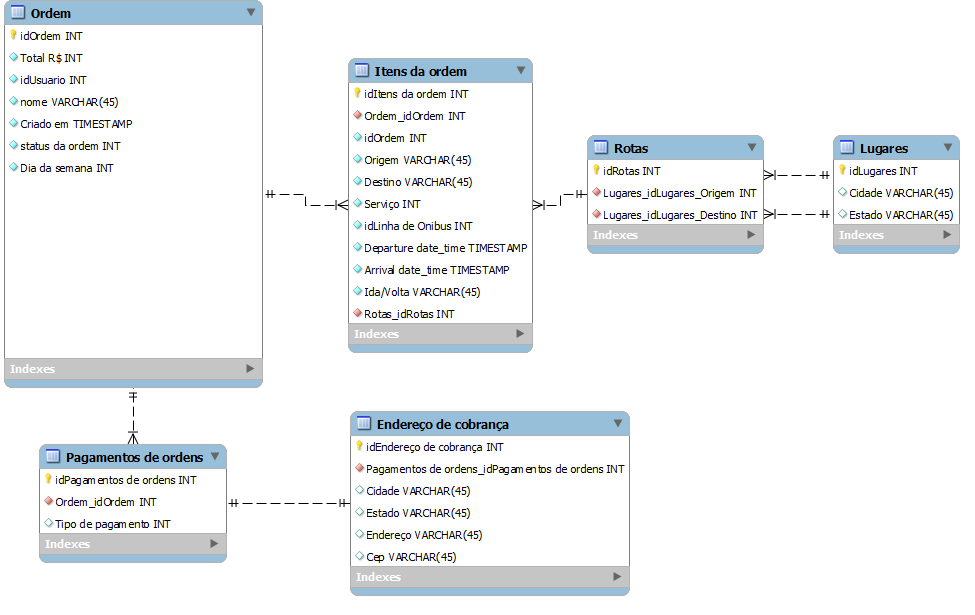
\includegraphics[width=1\textwidth]{../img/estrutura-banco-de-dados}
    \caption{Relacionamento entre as tabelas do banco de dados de passagens de ônibus}
    \label{fig:bd-clickbus}
\end{figure}
\end{center}
\end{frame}